\section{Introduction} \label{sec:intro}
In paravirtualization~\cite{XEN-SOSP03,whitaker2002scale}, the operating system of each Virtual Machine (a.k.a. guest or guest domain) and the hypervisor share the same virtual space.
In order to prevent malicious accesses from the guest OS, the hypervisor sets the guest page tables read-only, and intercepts and validates the updates to ensure that there is no runtime violation~\cite{XEN-SOSP03}.
However, only the page table based protection is not enough to defend against the DMA attacks driven by the malicious guest OS~\cite{disaggregation}.
To fix this gap, the hypervisor resorts to the I/O virtualization (AMD-Vi~\cite{amdvt} or Intel VT-d~\cite{intelvt}) technology, which leverages a new Input/Output Memory Management Unit (IOMMU) to restrict DMA accesses on the physical memory pages occupied by the hypervisor and the guest page tables.
% talk about the security protection in software and dma aspects
To integrate the above protection techniques, the guest page table management and the hypervisor are required to be properly patched.

\begin{figure*}[ht]
\centering
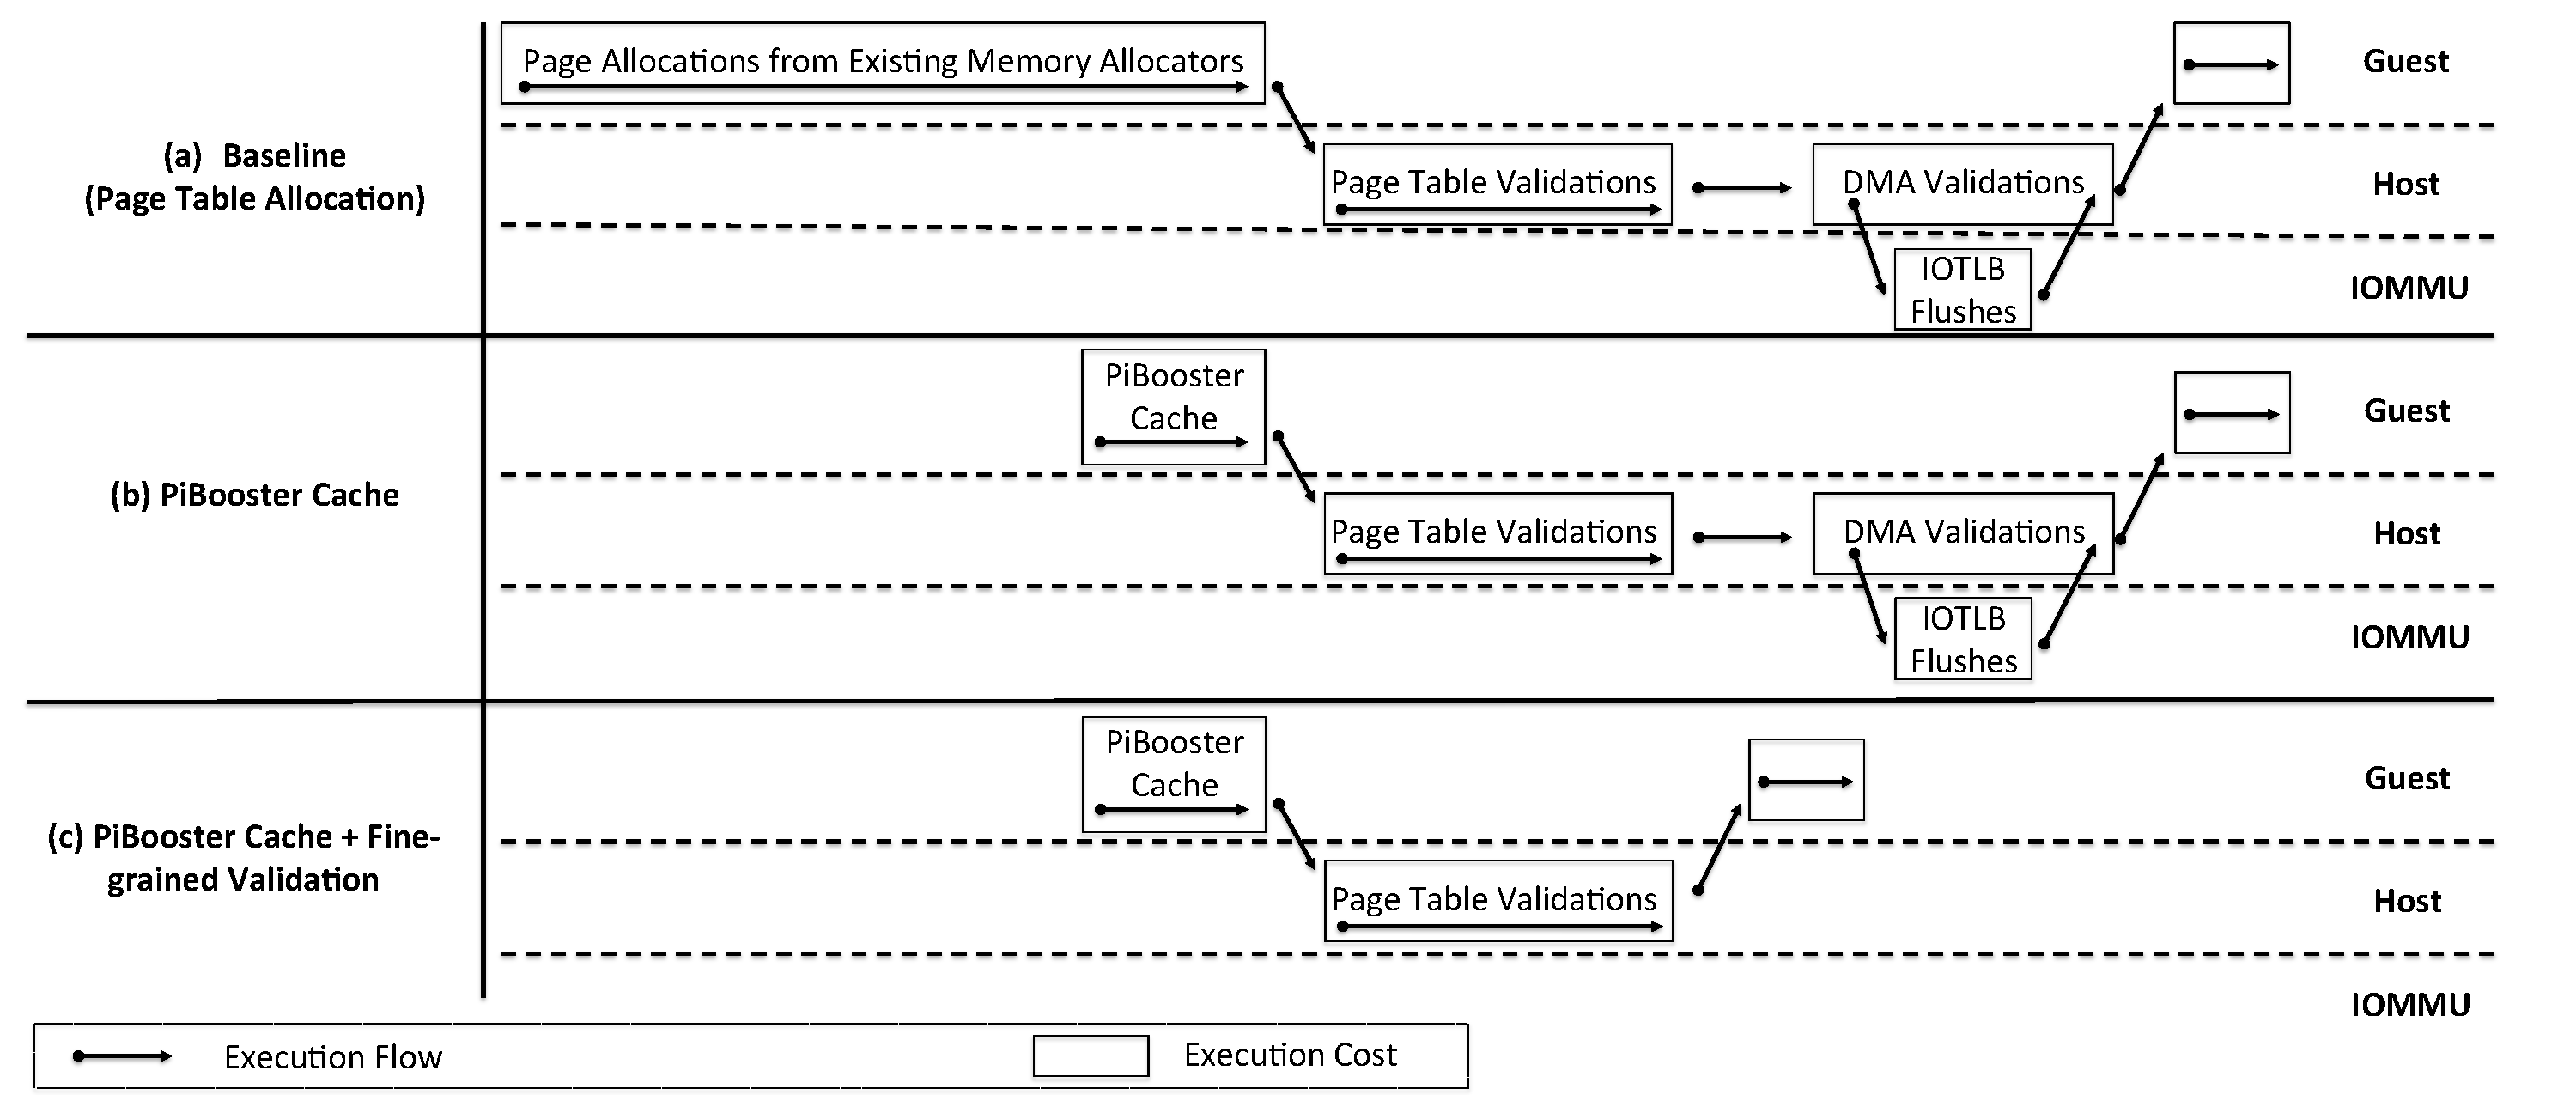
\includegraphics[width=0.9\textwidth]{image/overview/overview.pdf} \\
\caption{Solution Overview. When the \name cache and fine-gained validation mechanisms are enabled,
the execution path of page table allocation is dramatically reduced, and the additional IOTLB flushes are eliminated.}
\label{fig:overview}
\end{figure*}

%Highlight the problem, and emphasize the importance.
\mypara{Problem}
However, all existing patches mainly focus on the security enhancements of the hypervisor, without enough attentions to the performance improvements, which results in two noticeable issues.
The first one is the long execution paths of the guest page table (de)allocations, which involve the complex memory allocation process and the additional security validation procedure.
The memory allocation process frequently involves the \emph{slab} allocator~\cite{slaballocator} and the page frame allocations that are frequently managed with a buddy system~\cite{buddyallocator}, which introduces deep invocations for each page-table (de)allocation.
Moreover, the additional security validation procedure always adds extra costs for preventing malicious software and DMA accesses.
All these lead to poor performance of the page table (de)allocation, and consequently result in the long latencies of the creations and exits of processes.

The other one is the additional IOTLB flushes introduced by the security validations of the page table (de)allocations.
The guest page tables should be non-readable for any DMA requests and the corresponding pages should be readable and writable when the page tables are released.
The updates of the access permissions require IOTLB flushes to refresh the access permissions, which is necessary for the sake of the security of the hypervisor.
In addition, these access permission update events are \emph{often} triggered during the whole life cycle of a running system.
As a consequence, the IOTLB flushing events are \emph{frequently} involved, which inevitably increases the IOTLB miss rate and lowers the speed of the DMA address translation.
All these are likely to introduce negative impacts on the I/O performance of all peripheral devices.
The baseline of Figure~\ref{fig:overview}a illustrates the two issues in the page table allocation process.

\mypara{Solution}
%introduce our approach
The above identified performance issues urge us to revise the design of the page table management to improve the performance and keep the security guarantees.
In response to the appeal, in this paper we propose \name, a novel software-only approach for improving performance in page table management.
First, \name shortens the execution paths of the page table (de)allocations by \cache, which maintains a dedicated buffer for serving page table (de)allocations (Figure~\ref{fig:overview}b).
The \cache queues the deallocated page-table pages in the hope that
they will be reused (popped out of the cache) in the page table allocations in the near future.
By doing so, the page table allocations do not need to involve the costly memory management subsystem every time, instead they could directly get pages from the cached buffer.
As the functionalities of the \cache are concentrated, it is relatively easy to make it small, simple and efficient, dramatically shortening the execution path.

Second, \name eliminates the additional IOTLB flushes with a fine-grained validation scheme (Figure~\ref{fig:overview}c ), which separates the DMA and software validations.
In the original design, there are two types of pages: writable page that is writable for software and DMA requests, and non-writable page (e.g., page-table page) that are non-writable for both software and DMA.
The page table allocations and deallocations always involve the type changes between both of them.
Thus, the hypervisor has to do both software and DMA validations to ensure that both of them are not violating the security policies.
However, we observed that it is not necessary to do DMA validation every time if we create a new page type (i.e., semi-writable page) with non-writable permission for DMA access, and make the page type changes are only happened between the page-table pages and the semi-writable pages during the page table allocations and deallocations.
In addition, the semi-writable pages can be smoothly maintained by the \cache.

We implement a prototype on Xen with Linux as the guest kernel. We do small modifications of Xen version 4.2.1 ($166$ SLoC) and Linux kernel version 3.2.0 ($350$ SLoC).
We evaluate the I/O performance in both micro and macro ways.
The micro experiment results indicate that \name is able to completely eliminate the additional IOTLB flushes, and effectively reduces (de)allocation time of the page table.
There are (34\%, 47\%), (38\%, 22\%) and (65\%, 65\%) improvements for a pair of allocation and deallocation for three-level page table, from top to bottom. 
Even in the worst cases when the \name has to go through the traditional path to allocate pages, the performance overhead for one page table allocation is still very small, only adding about 20 instructions. Fortunately, the worst cases are rarely happened. According to our experiment results, the number of worst cases is only $348$, out of the total allocation requests (i.e., $198990$), in 30 minutes execution.  
The macro benchmarks show that \name has no negative impact on the CPU computation, network I/O and disk I/O.
In particular, the latencies of the process creations and exits are expectedly reduced by 24\% on average.

In summary, we make the following contributions:
\begin{enumerate}
\item We identify two significant performance issues in the page table management. In particular, we are the first, to the best of our knowledge, to identify the performance issue between guest page table (de)allocations and the IOTLB flushes.
\item We proposed a novel approach - called \name, to shorten the execution paths of the page table allocation and deallocations, and eliminate the additional IOTLB flushes, without sacrificing the system security.
\item We implemented a prototype of the page table cache and evaluated the performance in both micro and macro ways. The experiment results indicate the \name can benefit the page table (de)allocations, without no negative performance impacts on the system.
\end{enumerate}

The rest of the paper is structured as follows: In Section~\ref{sec:prob}, we briefly describe the background knowledge, and highlight the performance issues. Then we describe the system overview and implementation in Section~\ref{sec:overview} and Section~\ref{sec:impl}. In Section~\ref{sec:eva}, we evaluate the performance of the \name system, and discuss several issues in Section~\ref{sec:dis}. At last, we discuss the related work in Section~\ref{sec:related}, and conclude the whole paper in Section~\ref{sec:con}.

